\section{Formal Description and Analysis of \seccells' 
Userspace Instructions}
\label{app:instructions}

We define the semantics of \seccells' unprivileged instructions
in \autoref{fig:seccell_ops_formal} and discuss their corresponding
security checks below.

\paragraph{\sdswitch}
This instruction checks that the jump target is valid, and holds
an \sdentry instruction executable by the target \secdiv.
With the precondition that the caller \secdiv does not have
writable permission to any \cell executable by the target \secdiv,
\sdswitch guarantees compartment entry at previously defined entry 
points (helping implement call gates). 

\paragraph{\scprot}
This instruction checks that the target \cell is accessible by the
\secdiv, and the new permissions are a subset of the existing permissions.
After this instruction, the \secdiv is assured to have no more permissions
than before.

\paragraph{\scgrant, \screcv and \sctfer}
\scgrant checks that the granting \secdiv has permissions to the
\cell, and that the granted permissions are a subset of its existing
permissions.
\screcv, in turn, checks that the \secdiv is receiving permissions for a
valid cell, that the permissions were previously granted by the
specific \secdiv that the receiving \secdiv expects, and that the received
permissions are a subset of the permissions granted.
\sctfer includes the checks of both \scgrant and \scprot.
The granting and receiving \secdiv{}s must cooperate in order to
transfer permissions, and together finish with the same or fewer
permissions than they began with.

A correct compartment is defined to not grant or receive any permissions 
or invalidate cells that it is not required to grant as per a correct
compartmentalization policy.
Considering a set of compromised attacker \secdiv{}s and their permissions 
to \cell{}s and assuming that uncompromised compartments are correct,
\seccells guarantees that the attackers can neither gain any new permissions 
through any sequence of permission transfer instructions 
nor elevate the permissions of any uncompromised compartment.
Using \scgrant and \screcv instructions, the compromised compartments can
transfer permissions between themselves but those grants cannot include 
permissions which none of the attackers had initially.
The only way for the attackers to gain permissions is from
an uncompromised \secdiv either granting permissions to a \cell or from 
invalidating a private \cell which one of the attackers can validate with \screval.
The only way for the attackers to inject permissions is to have an
uncompromised \secdiv receive them.
By definition, uncompromised compartments will do neither of the above.
Once again, we stress on the importance of a correct compartmentalization
policy.
No mechanism, including \seccells, can protect against an insecure policy
where compartments transfer permissions from/to untrusted compartments
without proper validation.

\paragraph{\scinval} 
This instruction allows a \secdiv to invalidate a \cell to which
it has exclusive access, and to which no outstanding permission grants
exist.
The first condition can be true for a private region, or for one
which other \secdiv{}s have willingly dropped permissions.
Consequently, no other \secdiv will unwittingly lose permissions to
the invalidated \cell as a consequence of \scinval.
The second condition provides the assurance that no compartment can
regain permissions to the cell without executing \screval.

\paragraph{\screval} 
This instruction checks that the address corresponds to an existing 
\cell{} and that it is currently invalid. 
Due to the initial invalidity of the \cell, no \secdiv{}s could have
access to the cell to be revalidated.

\paragraph{\scexcl}
This instruction does not modify any permissions, only allowing a
\secdiv{} to check if it has exclusive access to a \cell{} to which
it already has access to.

\begin{comment}
\section{Memory layout of the unified \ptable-\gtable}
\label{app:ptable}

\autoref{fig:ptable_layout} shows the detailed implementation of the
unified \ptable-\gtable.

The table contains a sorted list of cell descriptors, including a
metadata ``cell'' used for storing its sizing parameters.
As described in \autoref{sec:seccells:impl}, each cell descriptor stores virtual 
and physical frame numbers uniquely identifying a VMA, as well as a 
validity flag to track the cell's current validity.
The metadata cell tracks the number of allocated \cell{}s ($N$), the
number of \secdiv{}s ($M$), and sizing factors $T$ (upper bound on \cell count)
and $R$ (upper bound on \secdiv count).
When software requires additional \secdiv{}s or \cell{}s, it must request
the supervisor via a system call.
If the request overflows the bounds imposed by factors $R$ and $T$, the
supervisor must resize this table as required.
The \cell descriptor list is followed by the \ptable, and then by the
\gtable.

\atri{Show how the limits on number of cells and secdivs is determined}

\begin{figure*}
  \centering
  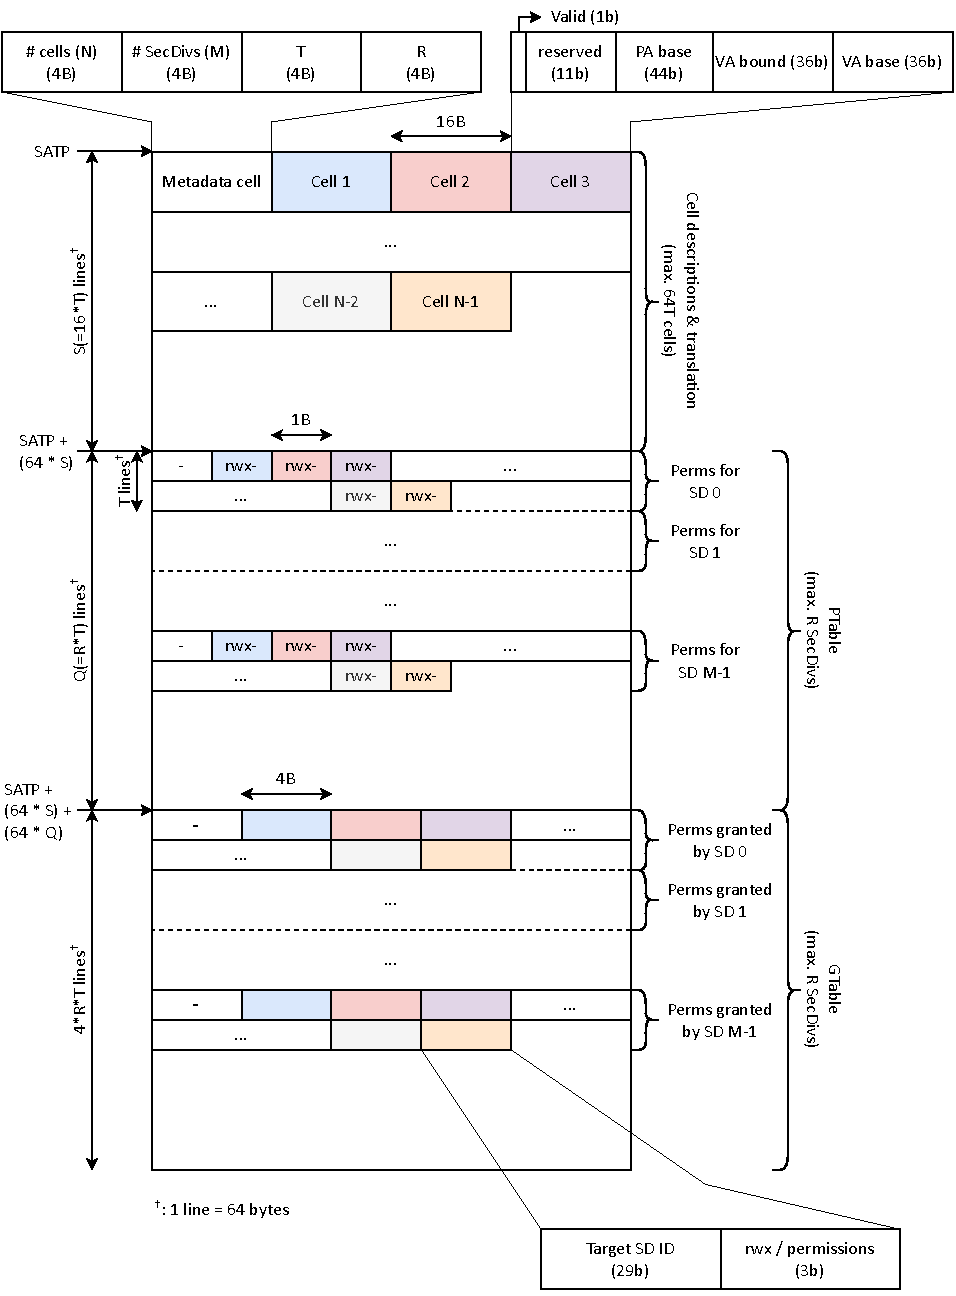
\includegraphics[height=0.95\textheight]{media/seccells/ptable_layout.pdf}
  \caption{Layout of the unified \ptable-\gtable.}
  \label{fig:ptable_layout}
  %\Description[<short description>]{<long description>}
\end{figure*}
\end{comment}

\section{Justification for \autoref{tab:req_comparison}}
\label{app:justification_table1}

\paragraph{Obj. \req{1a}}
MPK, ERIM and Donky do not check permissions for instruction fetches, 
simplifying code injection.
Under our threat model, an attacker can inject \Code{wrpkru} instructions 
to corrupt permissions.

\paragraph{Obj. \req{1b}}
Through code injection, call gates in MPK and ERIM can be bypassed.

\paragraph{Obj. \req{1c}}
CODOM requires migrating threads without context isolation.
MPK, ERIM and Donky rely on call gates if context isolation is desired.
However, MPK and ERIM cannot enforce call gates under our threat model.
Donky gives no mechanism for a compartment to restore its state without
trusting general-purpose registers. 
Further, Donky cannot adopt a \seccells-like software approach because a 
compartment has no way to identify itself.

\paragraph{Obj. \req{1d}}
CHERI allows one compartment to unilaterally send a capability to another compartment, 
unchecked by the TCB and unacknowledged by the receiver.

\paragraph{Obj. \req{1e}}
No mechanism except XPC considers the challenge of exclusive access.

\paragraph{Obj. \req{1f}}
A compartment in MPK and ERIM cannot check the value of the \Code{pkru}
register for another compartment, hindering audits.
Cross-core \Code{pkru} reads are not possible.
CHERI requires an expensive full memory scan for capabilities to perform
an audit.

\paragraph{Obj. \req{2a}}
Page-table based translation and permission checking encounter TLB-reach
limits leading to multi-cycle common case access verification for many
widely-used programs including \Code{memcached}. The mechanisms relying on
such page tables for either translation or permission checking fail this
requirement.

\paragraph{Obj. \req{2b}}
Supervisor-mediated cross-compartment calls in UNIX-like OSs,
Mondrian, lwC and CHERI require 100s or 1000s of cycles to complete.

\paragraph{Obj. \req{2c}}
Supervisor-mediated permission transfers are slow (UNIX, MMP, lwC).
MMP proposes the use of redundant mappings with different permissions
to implement a form of zero-copy transfer which is not generic.
CODOM does not really support permission transfers.
XPC restricts permission transfer to a single relay segment.

\paragraph{Obj. \req{3a}}
CODOM identifies the executing compartment by the instruction pointer, 
limiting the flexibility to share code/data regions between compartments.

\paragraph{Obj. \req{3b}}
UNIX, MMP, lwC, XPC and CHERI cannot eliminate context switching when a
permissive policy allows migrating threading between compartments.

\section{Existing mechanisms with \seccells}
\label{app:integrate_exist}
Many existing performance or security mechanisms can be integrated with
\seccells, either unmodified or with modifications described in this section.

\paragraph{Physical Memory Protections}
\seccells enforces permissions on the virtual address space, and is therefore
trivially compatible with physical memory protection schemes 
including RISC-V's Physical Memory Protection (PMP) mechanism, 
processor reserved memory for Intel's SGX
and vendor-specific protections like Qualcomm's XPU~\cite{qualcomm_ac}.
These mechanisms will apply to the physical address output by 
\seccells' MMU after \ptable access control checks.

\paragraph{Pointer authentication and capabilities}
ARM's pointer authentication code (PAC) feature and CHERI's capabilities
improve memory safety by protecting pointers from illegal 
modifications (overwriting when stored in memory and out-of-bound
increment respectively). Both mechanisms are orthogonal to,
and can integrate with \seccells, which checks accessess against \ptable
permissions when the 
pointers protected by these mechanisms are finally dereferenced, providing
another layer of protection against attacks like PACMAN~\cite{pacmanRavichandranNLY22}.

\paragraph{Hardware and Software Control Flow Integrity}
Hardware (e.g., Intel CET) and software (e.g., LLVM-CFI) control-flow
protections can integrate with \seccells, 
improving intra-compartment control-flow protection to
complement \seccells' inter-compartment call gates (\sdentry).
CET can continue to check indirect call targets for \Code{endbr} instructions. 
LLVM's and other fine-grained CFI pointer checks are implemented in software, 
orthogonal to hardware control flow checks.


\paragraph{Page-based mechanisms}
By itself, \seccells restricts popular mechanisms (e.g., guard pages, swapping)
operating on pages and page tables since translations and protections are 
tracked at \cell granularity.
However, \seccells can be integrated with upcoming intermediate address-space 
systems like Midgard re-enabling programmers to implement these crucial 
features.
Midgard couples \seccells-like range-based translation at the core with
a second level of page-granularity translations at the backside of the 
last-level cache.
Guard pages and swapping can both be implemented by unmapping the requisite pages 
in the backside translation.


\section{Speculative Side-Channel Attacks}
\label{app:sidechannel}

We consider the threat of speculative side-channel attacks like 
Spectre~\cite{KocherHFGGHHLM019}
in \seccells' design, despite omitting such attacks from our attacker model.
\seccells{} introduces additional mechanisms for changing an executing
thread's permissions, through userspace compartment switching and
permission transfers.
Fault-based attacks like Meltdown~\cite{lipp18sec} must be prevented in
implementations by preventing faulting loads from accessing memory or
forwarding their data to subsequent instructions~\cite{WeisseNLWK19}.

\seccells specifies that userspace instructions are serializing, 
precluding speculative permission changes.
An attacker cannot, for example, speculatively switch to a victim
\secdiv using an \sdswitch following a long-latency branch and read 
the victim's private data using the victim's permissions.
\seccells' permission transfer instructions are atomic, preventing visibility 
or exploitation of any intermediate permission state.
An attacker \secdiv cannot, for example, drop permissions for a \cell
using \scprot while transferring the same permissions using \sctfer in parallel.
Our firmware (and future microcode) implementation use load-linked 
store-conditional atomic operations commonly available across architectures
to ensure atomicity.
\seccells allows the pipeline to speculate as usual within a compartment's 
execution, and speculative accesses are also subject to access control 
by the MMU and cannot illegally access any \cell.
Access control, therefore, also limits the leakage potential of existing
Spectre gadgets.
Whereas a Spectre gadget on a traditional processor can address and
access any user memory in the process' address space, the same Spectre
gadget can only access memory within the compartment's \cell{}s.
\seccells also limits the code (speculatively) executable within a compartment,
further restricting the availability of Spectre gadgets.

\section{\seccells Implementation Trade-Offs}
\label{app:impl_options}

\seccells permits a range of implementations scaling from simple 
microcontrollers with firmware emulation for added userspace
instructions to server grade processors with microcode or hardware 
implementations. In this section, we describe the trade-offs and 
justify our implementation in \autoref{sec:seccells:impl}.

\paragraph{Firmware}
On the simplest side of the spectrum, instructions can be emulated
by firmware using trap-and-emulate.
Firmware is programmable code which runs in a privileged execution mode 
and uses native ISA instructions.
\seccells' instructions will trap into firmware, and be dispatched to 
the emulation code.
Firmware implementations are cheap, requiring no additional hardware, but 
slower than alternate implementations.
For the simple RISC-V RocketChip microcontroller, we choose 
firmware emulation for permission transfer instructions.
Note that the firmware can also forward traps to be emulated by
either the supervisor or even a privileged userspace library.
However, the additional security risk of emulation by less trusted
software risk and the overhead of forwarding traps makes such
implementations less attractive.

\paragraph{Hardware}
Alternatively, instructions can be implemented in hardware with 
finite-state machine circuits.
While this design option implies better performance,
designing complex hardware comes with silicon and power costs and
substantial complexity.
Hardware bug fixes incur the significant cost of the tape-out process.
Server and desktop processors generally include beefy cores with
large silicon area, where hardware implementations may match the
processor's targeted performance.
We implement the crucial \sdswitch instruction in hardware
to reap the performance advantage,
and because of the simplicity of its design.

\paragraph{Microcode}
A third option, microcode, is programmable code provided by the 
processor manufacturer, built from low level operations including ones 
not available through the ISA interface.
When a instruction implemented in microcode is encountered, a microcode
sequencer fetches microcode from an on-chip RAM and executes them in the
pipeline.
Microcode eliminates the cost of trapping and dispatch encountered in 
firmware emulation ($77\%$ of the latency of emulating \scprot),
and can also leverage hardware-specific optimizations.
Microcode is popular for implementing complicated instructions
with high performance like SGX's \Code{EENTER}/\Code{EEXIT} instructions.
Microcode also has the advantage of being programmable, and have been
leveraged to fix processor errata and bugs.
While the simple RocketChip lacks a microcode sequencer, 
we envision microcode to be ideal for implementing \seccells'
permission transfer instructions for high-performance processors.



TODO: Put details of SecureCells implementation (bits of instructions, etc.)